\subsection{Motivation}

\begin{frame}
  \frametitle{Nuclear Security}
  Slide on nuclear security in general \\~\\ 

  The nuclear security enterprise instead focuses on preventing or mitigating
  undesirable outcomes of a different variety, like nuclear terrorism. Nuclear
  security's goal is keeping all of the nuclear material in the world inside a
  regulatory pipeline, so none of it gets into the hands of people who want to
  do others harm

\end{frame}

\begin{frame}
  \frametitle{Nuclear Forensics}
  \begin{figure}
    \centering
    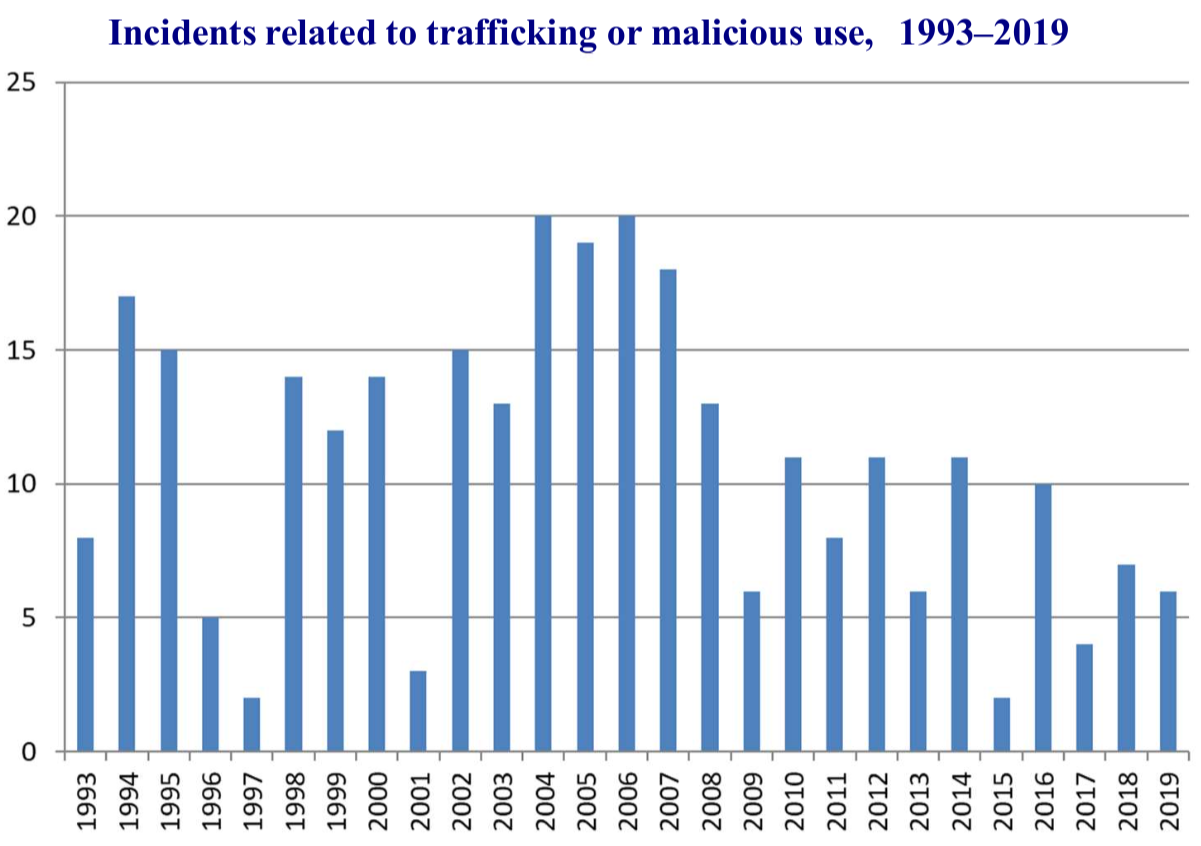
\includegraphics[width=0.78\textwidth]{./figures/nucleartrafficking.png}
  \end{figure}
  Incidents of highest concern: Highly enriched uranium (12), plutonium (2), 
  plutonium-beryllium neutron sources (5) \cite{itdb}
\end{frame}

\begin{frame}
  \frametitle{Nuclear Forensics Investigations}
  Slide on timeline of nuclear forensics investigation\\~\\
  Tradeoff of time and information
\end{frame}

\begin{frame}
  \frametitle{Main Goal}

  Is it possible to \textbf{speed up} a nuclear forensics
  \textbf{investigation} of spent nuclear fuel with \textbf{field-deployable
  detection}?

\end{frame}

\begin{frame}
  \frametitle{Statistical Methods}

  Why are statistical methods being used

\end{frame}

\subsection{Background}

\begin{frame}
  \frametitle{Nuclear Forensics Investigations}
  \begin{adjustwidth}{-10pt}{0pt}
  \begin{figure}
    \centering
    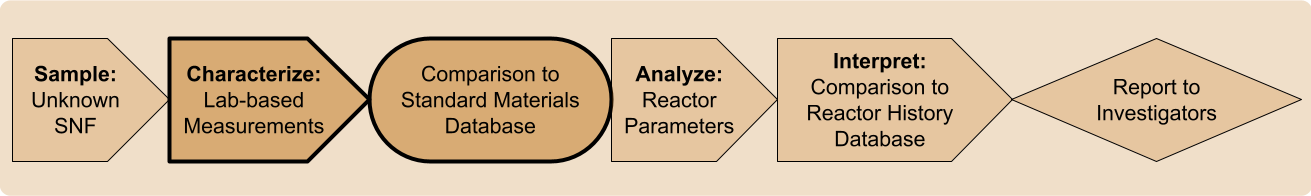
\includegraphics[width=\textwidth]{./figures/forensicsrealworld.png}
  \end{figure}
  \vspace{-3mm}
  \begin{minipage}[t]{0.5\textwidth}
    \begin{block}{Pre-detonation}
      \begin{itemize}
        \item<1-> Collection: depends on intercepted material
        \item<2-> Characterization: non-destructive and destructive
        \item<3-> Goals:
        \begin{itemize}
          \item Inverse problem: material chain of custody
          \item Safety: material handling and security
        \end{itemize}
        \item<4-> Data evaluation
      \end{itemize}
    \end{block}
  \end{minipage}%
  \hfill
  \begin{minipage}[t]{0.5\textwidth}
    \begin{block}{Post-detonation}
      \begin{itemize}
        \item<1-> Collection: debris, swipe samples
        \item<2-> Characterization: rapid analysis of isotope ratios
        \item<3-> Goals
        \begin{itemize}
          \item Inverse problem: reconstruct weapon design/yield
          \item Safety: informing disaster response
        \end{itemize}
        \item<4-> Data evaluation
      \end{itemize}
    \end{block}
  \end{minipage}
  \end{adjustwidth}
\end{frame}

\begin{frame}
  \frametitle{Nuclear Forensics Investigations}
  \vspace{-5mm}
  \begin{figure}
    \centering
    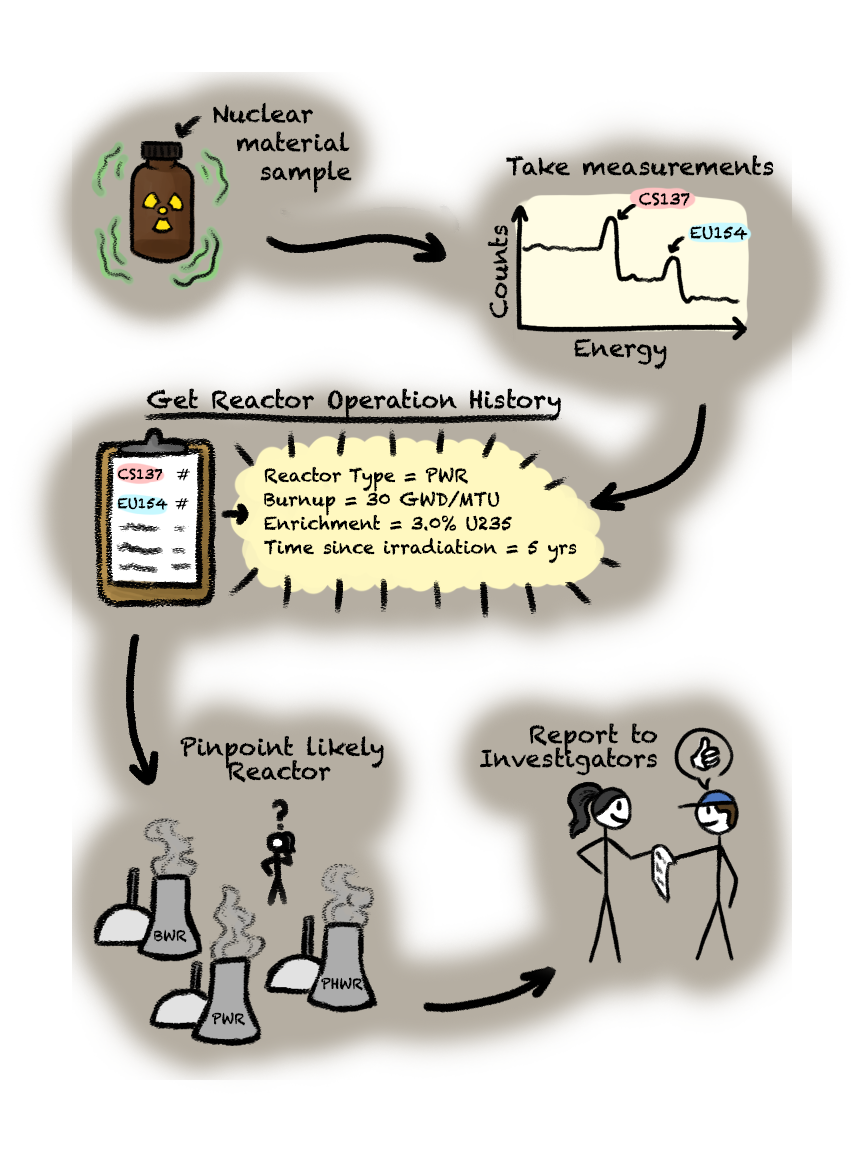
\includegraphics[height=0.98\textheight]{./figures/nf-workflow.png}
  \end{figure}
\end{frame}

\begin{frame}
  \frametitle{ML Intro}
  Short ML intro
\end{frame}

\begin{frame}
  \frametitle{Supervised Regression: Training and Predicting}
  \begin{figure}
    \centering
    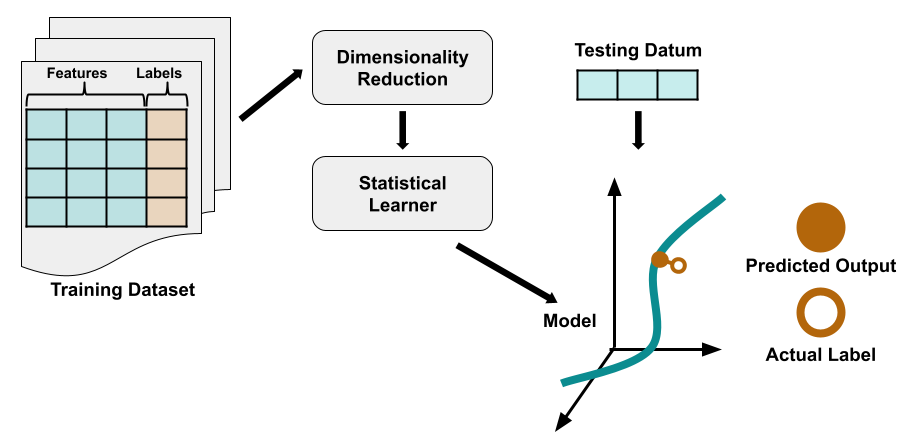
\includegraphics[width=\textwidth]{./figures/SupervisedRegression.png}
  \end{figure}
\end{frame}

\begin{frame}
  \frametitle{Introduction Summary}
  NF, needs\\
  ML, usefulness\\
  Main goal, speed
\end{frame}

